\documentclass{report}
    \title{\vspace{-50pt}\textbf{\underline{COP4620 Notes}}}
    \author{}
    \date{}
    \addtolength{\textheight}{3cm}
    \usepackage[tmargin=1in,lmargin=1in,rmargin=1in]{geometry}
    \usepackage[T1]{fontenc}
	\usepackage{titlesec}
    \usepackage{makecell}
    \usepackage{longtable}
    \usepackage{multicol}
    \usepackage{soul}
    \usepackage{tikz}
	\usepackage{hyperref}
    \renewcommand\theadfont{\bfseries\sffamily}
    \usetikzlibrary{automata, positioning, arrows, babel,positioning,shapes}
    \tikzset{
        ->, % makes the edges directed
        >=stealth', % makes the arrow heads bold
        node distance=3cm, % minimum distance between two nodes. Change if necessary.
        every state/.style={thick, fill=gray!10}, % sets properties for each state node
        initial text=$ $, % sets the text that appears on the start arrow
    }

    
	\hypersetup{
    colorlinks=true,
    linkcolor=blue,
    filecolor=purple,      
    urlcolor=cyan
    }
    
	\titleformat{\chapter}[display]
	{\bfseries\Large\itshape}
	{Chapter\ \thechapter}{0.5ex}{ }

	\titleformat{\section}
	{\normalfont\bfseries}
	{\thesection}{0.5em}{}

	\titleformat{\subsection}
	{\normalfont\bfseries}
	{\thesubsection}{0.5em}{}

    \titlespacing\chapter{0pt}{12pt plus 0pt minus 4pt}{0pt plus 0pt minus 4pt}
    \titlespacing\section{0pt}{12pt plus 4pt minus 8pt}{0pt plus 2pt minus 8pt}
    \titlespacing\subsection{0pt}{12pt plus 4pt minus 4pt}{0pt plus 2pt minus 4pt}
    \titlespacing\subsubsection{0pt}{12pt plus 4pt minus 2pt}{0pt plus 2pt minus 2pt}

%    \setlist[description]{noitemsep, topsep=0pt, itemsep=-.1em}
%    \setlist[enumerate]{noitemsep, topsep=0pt, itemsep=-.1em}
%    \setlist[itemize]{noitemsep, topsep=0pt, itemsep=-.1em}
%   \setlist[trivlist]{noitemsep, topsep=-8pt, itemsep=-.1em}

    \newcommand{\comment}[1]{}
\begin{document}

\maketitle
\tableofcontents

\chapter{Top Down Parsing Lecture 2-2-2022}

\section{First Sets}
First set ( beginning terminals) set of terminal and non-terminal, with empty string.
It is the first terminal in a production. If the first one contains lambda move to the next until last symbol or, no lambda or symbols. Top down uses leftmost derivation. We do not care about non-terminals - we want the set terminals!!!!!

\subsection{A Simple Example - Slides 4 - 15}
\vspace{-1.5em}
\begin{multicols}{2}
  \begin{enumerate}
    \setlength\itemsep{-.25em}
    \item S $\rightarrow$ ABc\$
    \item A $\rightarrow$ xaA
    \item A $\rightarrow$ yaA
    \item A $\rightarrow$ c
    \item B $\rightarrow$ b
    \item B $\rightarrow$ $\lambda$\newline
  \end{enumerate}
  \setlength{\leftskip}{-12em}
  First (A) = First(xaA) $\cup$ First(yaA) $\cup$ First(c)\newline
  \indent\hspace{2cm}2\hspace{5.5em}3\hspace{5.5em}4\newline
  \indent\hspace{.25cm}First (xaA) = First of \{x\} - $\lambda$ = \{x\} - $\lambda$ = \{x\}\newline
  \indent\hspace{.25cm}First (yaA) = First of \{y\} - $\lambda$ = \{y\} - $\lambda$ = \{y\}\newline
  \indent\hspace{.25cm}First (c) = \{c\}\newline
  First (A) = \{x\} $\cup$ \{y\} $\cup$ \{c\} = \{x, y, c\} $\leftarrow$ \textbf{Final set of A}\newline
  First (S) = First(ABc\$) = \{x, y, c\}
  \\
\end{multicols}

\vspace{-3em}

\subsection{Exercise - Slide 19}
\vspace{-1.5em}
\begin{multicols}{2}
  \begin{enumerate}
    \setlength\itemsep{-.25em}
    \item S $\rightarrow$ AB\$
    \item A $\rightarrow$ xaA
    \item A $\rightarrow$ yaA
    \item A $\rightarrow$ $\lambda$
    \item B $\rightarrow$ b\newline\newline
  \end{enumerate}
  \setlength{\leftskip}{-12em}
First (B) = First(b) = \{b\}  $\leftarrow$ \textbf{Final set of B}\newline
First (A) = First(xaA) $\cup$  First(yaA) $\cup$  First($\lambda$)\newline
\indent\hspace{.25cm}First (xaA) = First of \{x\} - $\lambda$ = \{x\} - $\lambda$ = \{x\}\newline
\indent\hspace{.25cm}First (yaA) = First of \{y\} - $\lambda$ = \{x\} - $\lambda$ = \{y\}\newline
\indent\hspace{.25cm}First ($\lambda$) = First of {$\lambda$} - $\lambda$ = \{$\lambda$\}\newline
First (A) = First(x) $\cup$  First(y) $\cup$  First($\lambda$)\newline
First (A) = \{x\} $\cup$  \{y\} $\cup$  \{$\lambda$\} = \{x, y, $\lambda$\} $\leftarrow$ \textbf{Final set of A}\newline
First (S) = First(AB\$) = (First(A) - $\lambda$) $\cup$ (\{b\} - $\lambda$) = \{x, y, b\} $\leftarrow$ \textbf{Final set}
\end{multicols}
\vspace{-1em}
\noindent\textbf{note:} *First of $\lambda$ is $\lambda$* -
First($\lambda$) = (First($\lambda$) - $\lambda$) = {$\lambda$} "reading $\lambda$" 

\subsection{In Class Quiz Q5 - Slide 25}
\vspace{-1.5em}
\begin{multicols}{2}
  \begin{enumerate}
    \setlength\itemsep{-.25em}
    \item S $\rightarrow$ AA\$
    \item A $\rightarrow$ xAy
    \item A $\rightarrow$ BB
    \item A $\rightarrow$ zB
    \item B $\rightarrow$ q
  \end{enumerate}
  \setlength{\leftskip}{-12em}
First (B) = First(zB) $\cup$ First(q) = \{z, q\}  $\leftarrow$ \textbf{Final set of B}\newline
First (A) = First(xAy) \newline
\indent\hspace{1cm}= \{x\} $\cup$ \{y\} $\cup$ \{q\} = \{x, y, q\} $\leftarrow$ \textbf{Final set of A}\newline
First (S) = \{x\} $\cup$ \{y\} $\cup$ \{q\} = \{x, y, q\} $\leftarrow$ \textbf{Final set of S}\newline
\{z, q\}, \{x, y, q\} and \{x, y, q\}\newline
\end{multicols}
\vspace{-1em}
\noindent\textbf{note:} you could have a \$ if it is the first, like $\lambda$\newline
\indent\hspace{.5cm}first sets are needed for everything, it will mess up parse table without

\section{Follow Sets}
\textbf{NO LAMBDA'S EVER!!!!}
All production beginning on the right hand side\newline
Follow set of S is the empty set
 - represents the entire string, so it will never have anything following!!!!

\subsection{Exercise - Slide 28}
\vspace{-1.5em}
\begin{multicols}{2}
  \begin{enumerate}
    \setlength\itemsep{-.25em}
    \item S $\rightarrow$ AB\$
    \item A $\rightarrow$ xaA
    \item A $\rightarrow$ yaA
    \item A $\rightarrow$ $\lambda$
    \item B $\rightarrow$ b\newline
  \end{enumerate}
  \setlength{\leftskip}{-12em}
Follow (S) = \{\}\newline
Follow (B) = First(\$) = \{\$\}  $\leftarrow$ \textbf{Final set of B}\newline
Follow (A) = First(B\$) $\cup$ Follow(A) $\cup$ Follow (A)\newline
\indent\hspace{.25cm}(First(B) - $\lambda$) = \{b\}\newline
\indent\hspace{.25cm}First(B\$) = \{b\}\newline
Follow (A) = \{b\} = \{b\} $\leftarrow$ \textbf{Final set of A}\newline
\end{multicols}

\newpage

\chapter{Top Down Parsing Lecture 2-7-2022}

\subsection{In Class Quiz Q6 - Slide 30}
\vspace{-1.5em}
\begin{multicols}{2}
  \begin{enumerate}
    \setlength\itemsep{-.25em}
    \item S $\rightarrow$ AA\$
    \item A $\rightarrow$ xAy
    \item A $\rightarrow$ BB
    \item A $\rightarrow$ zB
    \item B $\rightarrow$ q\newline\newline
  \end{enumerate}
  \setlength{\leftskip}{-12em}
Follow (S) = \{\} $\leftarrow$ \textbf{Final set of S}\newline
Follow (A) = First(A\$) $\cup$ Follow(\$) $\cup$ Follow (y)\newline
\indent\hspace{1.25cm}= (First(A)-$\lambda$) $\cup$ \{\$\} $\cup$ \{y\}\newline
\indent\hspace{1.25cm}= \{x, z, q\} $\cup$ \{\$\} $\cup$ {y}\newline
\indent\hspace{1.25cm}= \{x, z, q, y, \$\}			$\leftarrow$ \textbf{Final set of A}\newline
Follow (B) = First (B) $\cup$ Follow(A) $\cup$ \st{Follow (B)} $\leftarrow$ CROSS OUT FOLLOW(B)\newline
\indent\hspace{1.25cm}= \{z, q\} $\cup$ Follow(A)\newline
\indent\hspace{1.25cm}= \{x, z, q, y, \$\} 			$\leftarrow$ \textbf{Final set of B}
\end{multicols}
\vspace{-1em}
\textbf{MAKE SURE TO SHOW ALL WORK} including crossing out follows, etc


\section{Predict Sets}
\subsection{Exercise - Slide 32}
\vspace{-1.5em}
\begin{multicols}{2}
  \begin{enumerate}
    \setlength\itemsep{-.25em}
    \item S $\rightarrow$ AB\$
    \item A $\rightarrow$ xaA
    \item A $\rightarrow$ yaA
    \item A $\rightarrow$ $\lambda$
    \item B $\rightarrow$ b
  \end{enumerate}
  parse table LL(1) \textbf{abxy\$}\newline
  \begin{tabular}{|c|c|c|c|c|c|}
    \hline
	  & \thead{a} & \thead{b} & \thead{x} & \thead{y} & \thead{\$}\\
    \hline
	\textbf{S} &  & 1 & 1 & 1 & \\
    \hline
	\textbf{A} &  & 4 & 2 & 3 & \\
    \hline
	\textbf{B} &  & 5 &   &   & \\
    \hline
  \end{tabular}
  \newline\newline\newline\newline
  
\setlength{\leftskip}{-12em}
\hspace{-.5cm}Predict(1 S $\rightarrow$ AB\$) = \{x, y, b\}\newline
\indent\hspace{.25cm}First (B) = First(b) = \{b\} $\leftarrow$ \textbf{Final set of B}\newline
\indent\hspace{.25cm}First (A) = First(xaA) $\cup$  First(yaA) $\cup$  First($\lambda$) (from slide 19)\newline
\indent\hspace{1cm}First (xaA) = First of \{x\} - $\lambda$ = \{x\} - $\lambda$ = \{x\}\newline
\indent\hspace{1cm}First (yaA) = First of \{y\} - $\lambda$ = \{x\} - $\lambda$ = \{y\}\newline
\indent\hspace{1cm}First ($\lambda$) = First of \{$\lambda$\} - $\lambda$ = \{$\lambda$\}\newline
\indent\hspace{1cm}First (A) = First(x) $\cup$  First(y) $\cup$  First($\lambda$)\newline
\indent\hspace{1cm}First (A) = \{x\} $\cup$ \{y\} $\cup$  \{$\lambda$\} = \{x, y, $\lambda$\} $\leftarrow$ \textbf{Final set of A}\newline
\indent\hspace{.25cm}First(AB\$) = (First(A) - $\lambda$) $\cup$ First(B) = \{x, y, b\}$\leftarrow$ \textbf{Final set of AB\$} \newline
Predict(2 A $\rightarrow$ xaA) = \{x\}\newline
Predict(3 A $\rightarrow$ yaA) = \{y\}\newline
Predict(4 A $\rightarrow$ $\lambda$) = (First($\lambda$) - $\lambda$) $\cup$ Follow(A)				(from slide 28)\newline
\indent\hspace{2.3cm}= \{b\}\newline
Predict(5 B $\rightarrow$ b) = \{b\}
\end{multicols}


\subsection{An Example - Slide 36-37}
Stack-based parser for LL(1) \textbf{xayab\$}\newline
\begin{tabular}{|c|c|c|}
\hline
	\thead{Parse stack} & \thead{Remaining Input} & \thead{Parser action}\\
\hline
	S       & xayab\$ & predict 1\\
\hline
	AB\$   & xayab\$ & predict 2\\
\hline
	xaAB\$ & xayab\$ & match(x)\\
\hline
	aAB\$  & ayab\$   & match(a)\\
\hline
	AB\$  & yab\$   & predict 3\\
\hline
	yaAB\$ & yab\$   & match(y)\\
\hline
	aAB\$  & ab\$    & match(a)\\
\hline
	AB\$   & b\$     & predict 4\\
\hline
	B\$    & b\$    & predict 5\\
\hline
	b\$    & b\$    & match(b)\\
\hline
	\$     & \$     & done\\
\hline
\end{tabular}

\newpage

\subsection{In Class Quiz Q11 - Slide 43}
\vspace{-1.5em}
\begin{multicols}{2}
  \begin{enumerate}
    \setlength\itemsep{-.25em}
    \item S $\rightarrow$ AA\$
    \item A $\rightarrow$ xAy
    \item A $\rightarrow$ BB
    \item A $\rightarrow$ zB
    \item B $\rightarrow$ q\newline\newline
  \end{enumerate}
  \setlength{\leftskip}{-12em}
  predict(1. S $\rightarrow$ AA\$) = First(AA\$) = \{x, z, q\}\newline
  predict(2. A $\rightarrow$ xAy\$) = \{x\}\newline
  predict(3. A $\rightarrow$ BB\$) = \{z, q\}\newline
  predict(4. B $\rightarrow$ zB\$) = \{z\}\newline
  predict(5. B $\rightarrow$ q\$) = \{q\}\newline
\end{multicols}
\vspace{-2em}
  \begin{tabular}{|c|c|c|c|c|c|}
    \hline
	  & \thead{q} & \thead{x} & \thead{y} & \thead{z} & \thead{\$}\\
    \hline
	\textbf{S} & 1 & 1 &   & 1 & \\
    \hline
	\textbf{A} & 3 & 2 &   & 3 & \\
    \hline
	\textbf{B} & 5 &   &   & 4 & \\
    \hline
  \end{tabular}\newline\newline

\chapter{Bottom Up Parsing - Lecture 3 : 2-14-2022}

\section{LR Parsers}

\subsection{Configuration Closure Set}
Closure set - ( { S → .E\$} )

State 0
 = \{ S $\leftarrow$ \textbf{.}E\$, E $\leftarrow$ \textbf{.}E + T, E $\leftarrow$ \textbf{.}T, T $\leftarrow$ \textbf{.}ID, T $\leftarrow$ \textbf{.}(E) \}

\section{Characterstic Finite State Machine}
\vspace{-1.5em}  
\begin{multicols}{3}
\subsection{Example - Slide 11}
\noindent
  \begin{enumerate}
    \setlength\itemsep{-.25em}
    \item S' $\rightarrow$ S\$
    \item S $\rightarrow$ ID\newline\newline\newline\newline\newline\newline\newline
  \end{enumerate}
\subsubsection{State Diagram}
\noindent
  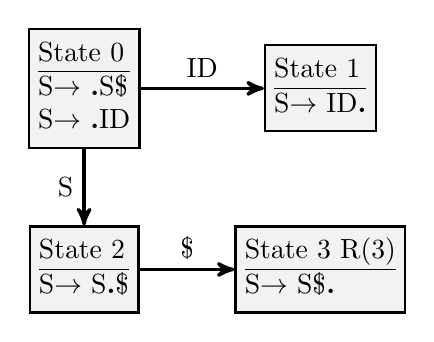
\begin{tikzpicture}
    \node[very thick, state, shape=rectangle] (0) {
    \makecell[l] {
    State 0 \\
    \hline
    S$\rightarrow$ \textbf{.}S\$ \\
    S$\rightarrow$ \textbf{.}ID
    }};
    \node[state, shape=rectangle, right of=0] (1) {
    \makecell[l] {
    State 1 \\
    \hline
    S$\rightarrow$ ID\textbf{.} \\
    }};
    \node[state, shape=rectangle, below of=0, yshift=7mm] (2) {
    \makecell[l] {
    State 2 \\
    \hline
    S$\rightarrow$ S\textbf{.}\$ \\
    }};
    \node[very thick, state, shape=rectangle, below of=1, yshift=7mm] (3) {
    \makecell[l] {
    State 3 R(3)\\
    \hline
    S$\rightarrow$ S\$\textbf{.}
    }};
    \draw[very thick]
          (0) edge[right, above] node{ID} (1)
          (0) edge[right, left] node{S} (2)
          (2) edge[right, above] node{\$} (3);
  \end{tikzpicture}
\subsubsection{GoTo/Action Table}
  \begin{tabular}{|c|c|c|c|c|c|}
    \hline
	  & \multicolumn{3}{c|}{Symbol} & Action Table\\
    \hline
	  & \thead{ID} & \thead{\$} & \thead{S} & \thead{Action}\\
    \hline
	\textbf{0} & 1 &   & 2 & Shift\\
    \hline
	\textbf{1} &   &   &   & Reduce 2\\
    \hline
	\textbf{2} &   & 3 &   & Shift\\
    \hline
	\textbf{3} &   &   &   & Accept R(1)\\
    \hline
  \end{tabular}
\end{multicols}


\subsection{Simple Example - Slide 13 or 20}
\vspace{-1.5em}  
\begin{multicols}{2}
\subsubsection{State Diagram}
\noindent
  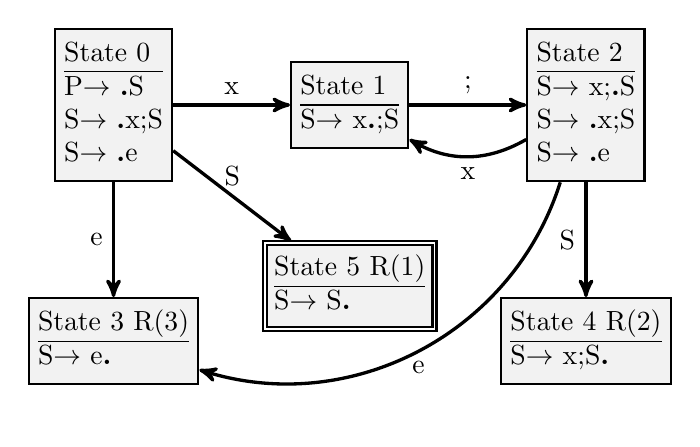
\begin{tikzpicture}
    \node[very thick, state, shape=rectangle] (0) {
    \makecell[l] {
    State 0 \\
    \hline
    P$\rightarrow$ \textbf{.}S \\
    S$\rightarrow$ \textbf{.}x;S \\
    S$\rightarrow$ \textbf{.}e
    }};
    \node[state, shape=rectangle, right of=0] (1) {
    \makecell[l] {
    State 1 \\
    \hline
    S$\rightarrow$ x\textbf{.};S \\
    }};
    \node[state, shape=rectangle, right of=1] (2) {
    \makecell[l] {
    State 2 \\
    \hline
    S$\rightarrow$ x;\textbf{.}S \\
    S$\rightarrow$ \textbf{.}x;S \\
    S$\rightarrow$ \textbf{.}e
    }};
    \node[very thick, state, shape=rectangle, below of=0] (3) {
    \makecell[l] {
    State 3 R(3)\\
    \hline
    S$\rightarrow$ e\textbf{.}
    }};
    \node[state, shape=rectangle, below of=2] (4) {
    \makecell[l] {
    State 4 R(2) \\
    \hline
    S$\rightarrow$ x;S\textbf{.} \\
    }};
    \node[state, accepting, shape=rectangle, below of=1, yshift=7mm] (5) {
    \makecell[l] {
    State 5 R(1) \\
    \hline
    S$\rightarrow$ S\textbf{.} \\
    }};
    \draw[very thick]
          (0) edge[right, above] node{x} (1)
          (0) edge[right, left] node{e} (3)
          (0) edge[right, above] node{S} (5)
          (1) edge[right, above] node{;} (2)
          (2) edge[bend left, below] node{x} (1)
          (2) edge[bend left=45, below] node{e} (3)
          (2) edge[right, left] node{S} (4);
  \end{tikzpicture}
\subsubsection{GoTo/Action Table}
  \begin{tabular}{|c|c|c|c|c|c|c|c|}
    \hline
	  & \multicolumn{5}{c|}{Symbol} & Action Table\\
    \hline
	  & \thead{x} & \thead{;} & \thead{e} & \thead{P} & \thead{S} & \thead{Action}\\
    \hline
	\textbf{0} & 1 &   & 3 &   & 5 & Shift\\
    \hline
	\textbf{1} &   & 2 &   &   &   & Shift\\
    \hline
	\textbf{2} & 1 &   & 3 &   & 4 & Shift\\
    \hline
	\textbf{3} &   &   &   &   &   & Reduce 3\\
    \hline
	\textbf{4} &   &   &   &   &   & Reduce 2\\
    \hline
	\textbf{5} &   &   &   &   &   & Accept R(1)\\
    \hline
  \end{tabular}
  \newline\newline
\end{multicols}

\vspace{-2.5em}
\begin{multicols}{2}
\subsubsection{Parser Table for String x;x;e}
\noindent
  \begin{tabular}{|c|c|c|c|}
    \hline
	\thead{} & \thead{Parse Stack} & \thead{Remaining} & \thead{Parser Action}\\
    \hline
	\textbf{1} & 0      & x;x;e & Shift 1 \\
    \hline
	\textbf{2} & 01     & ;x;e  & Shift 2 \\
    \hline
	\textbf{3} & 012    & x;e   & Shift 1 \\
    \hline
	\textbf{4} & 0121   & ;e    & Shift 2 \\
    \hline
	\textbf{5} & 01212  & e     & Shift 3 \\
    \hline
	\textbf{6} & 012123 &       & R(3) Goto State 4  \\
    \hline
	\textbf{7} & 012124 &       & R(2) Goto State 4  \\
    \hline
	\textbf{8} & 0124   &       & R(2) Goto State 5  \\
    \hline
	\textbf{9} & 05     &       & Accept State  \\
    \hline
  \end{tabular}
  \newline\newline
  \subsubsection{Parser Table for String x;x;x;e}
  \begin{tabular}{|c|c|c|c|}
    \hline
	\thead{} & \thead{Parse Stack} & \thead{Remaining} & \thead{Parser Action}\\
    \hline
	\textbf{1}  & 0        & x;x;x;e & Shift 1 \\
    \hline
	\textbf{2}  & 01       & ;x;x;e  & Shift 2 \\
    \hline
	\textbf{3}  & 012      & x;x;e   & Shift 1 \\
    \hline
	\textbf{4}  & 0121     & ;x;e    & Shift 2 \\
    \hline
	\textbf{5}  & 01212    & x;e     & Shift 1 \\
    \hline
	\textbf{6}  & 012121   & ;e      & Shift 2 \\
    \hline
	\textbf{7}  & 0121212  & e       & Shift 3 \\
    \hline
	\textbf{8}  & 01212123 &         & R(3) Goto State 4  \\
    \hline
	\textbf{9}  & 01212124 &         & R(2) Goto State 4  \\
    \hline
	\textbf{10} & 012124   &         & R(2) Goto State 4  \\
    \hline
	\textbf{11} & 0124     &         & R(2) Goto State 5  \\
    \hline
	\textbf{12} & 05       &         & Accept State  \\
    \hline
  \end{tabular}
\end{multicols}

\subsection{Shift Reduce conflict}
\vspace{-1.5em}
\begin{multicols}{2}
  \begin{enumerate}
    \setlength\itemsep{-.25em}
    \item S $\rightarrow$ Ay
    \item A $\rightarrow$ x
    \item A $\rightarrow$ xx\newline\newline\newline\newline\newline\newline\newline\newline\newline\newline\newline\newline
  \end{enumerate}
  \vspace{-80pt}
  \setlength{\leftskip}{-10em}
  \subsubsection{State Diagram}
  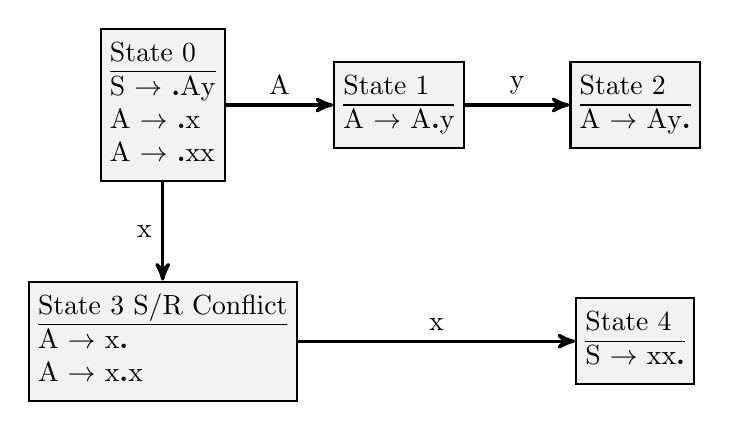
\begin{tikzpicture}
    \node[very thick, state, shape=rectangle] (0) {
    \makecell[l] {
    State 0 \\
    \hline
    S $\rightarrow$ \textbf{.}Ay \\
    A $\rightarrow$ \textbf{.}x \\
    A $\rightarrow$ \textbf{.}xx
    }};
    \node[state, shape=rectangle, right of=0] (1) {
    \makecell[l] {
    State 1 \\
    \hline
    A $\rightarrow$ A\textbf{.}y
    }};
    \node[state, shape=rectangle, right of=1] (2) {
    \makecell[l] {
    State 2 \\
    \hline
    A $\rightarrow$ Ay\textbf{.}
    }};
    \node[very thick, state, shape=rectangle, below of=0] (3) {
    \makecell[l] {
    State 3 S/R Conflict\\
    \hline
    A $\rightarrow$ x\textbf{.} \\
    A $\rightarrow$ x\textbf{.}x
    }};
    \node[state, shape=rectangle, below of=2] (4) {
    \makecell[l] {
    State 4 \\
    \hline
    S $\rightarrow$ xx\textbf{.} \\
    }};
    \draw[very thick]
          (0) edge[right, above] node{A} (1)
          (0) edge[right, left] node{x} (3)
          (1) edge[right, above] node{y} (2)
          (3) edge[right, above] node{x} (4);
  \end{tikzpicture}
\end{multicols}

\subsection{Quiz 6 - 11 States}
\vspace{-1.5em}
\begin{multicols}{2}
  \begin{enumerate}
    \setlength\itemsep{-.25em}
    \item S $\rightarrow$ AB\$
    \item A $\rightarrow$ xB
    \item A $\rightarrow$ xw
    \item B $\rightarrow$ xyA
    \item B $\rightarrow$ z
    \newline\newline\newline\newline\newline\newline\newline\newline\newline\newline\newline\newline\newline\newline
  \end{enumerate}
  \vspace{-50pt}
  \setlength{\leftskip}{-10em}
  \subsubsection{State Diagram}
  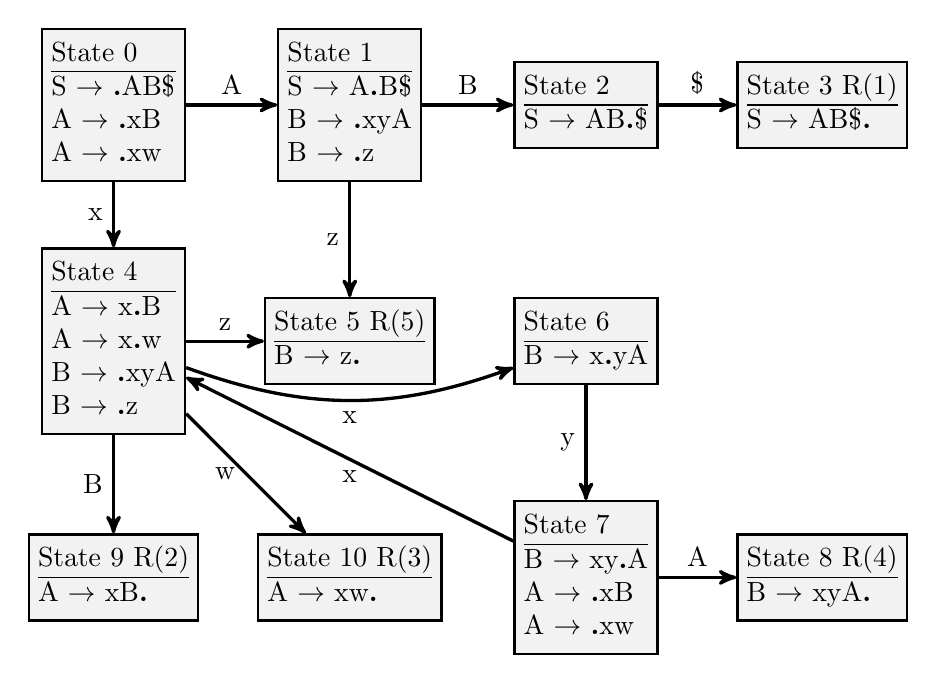
\begin{tikzpicture}
    \node[very thick, state, shape=rectangle] (0) {
    \makecell[l] {
    State 0 \\
    \hline
    S $\rightarrow$ \textbf{.}AB\$ \\
    A $\rightarrow$ \textbf{.}xB \\
    A $\rightarrow$ \textbf{.}xw
    }};
    \node[state, shape=rectangle, right of=0] (1) {
    \makecell[l] {
    State 1 \\
    \hline
    S $\rightarrow$ A\textbf{.}B\$ \\
    B $\rightarrow$ \textbf{.}xyA \\
    B $\rightarrow$ \textbf{.}z
    }};
    \node[state, shape=rectangle, right of=1] (2) {
    \makecell[l] {
    State 2 \\
    \hline
    S $\rightarrow$ AB\textbf{.}\$
    }};
    \node[state, shape=rectangle, right of=2] (3) {
    \makecell[l] {
    State 3 R(1)\\
    \hline
    S $\rightarrow$ AB\$\textbf{.} \\
    }};
    \node[very thick, state, shape=rectangle, below of=0] (4) {
    \makecell[l] {
    State 4\\
    \hline
    A $\rightarrow$ x\textbf{.}B \\
    A $\rightarrow$ x\textbf{.}w \\
    B $\rightarrow$ \textbf{.}xyA \\
    B $\rightarrow$ \textbf{.}z
    }};
    \node[state, shape=rectangle, below of=1] (5) {
    \makecell[l] {
    State 5 R(5)\\
    \hline
    B $\rightarrow$ z\textbf{.} \\
    }};
    \node[state, shape=rectangle, below of=2] (6) {
    \makecell[l] {
    State 6 \\
    \hline
    B $\rightarrow$ x\textbf{.}yA \\
    }};
    \node[state, shape=rectangle, below of=6] (7) {
    \makecell[l] {
    State 7 \\
    \hline
    B $\rightarrow$ xy\textbf{.}A \\
    A $\rightarrow$ \textbf{.}xB \\
    A $\rightarrow$ \textbf{.}xw
    }};
    \node[state, shape=rectangle, right of=7] (8) {
    \makecell[l] {
    State 8 R(4)\\
    \hline
    B $\rightarrow$ xyA\textbf{.} \\
    }};
    \node[state, shape=rectangle, below of=4] (9) {
    \makecell[l] {
    State 9 R(2)\\
    \hline
    A $\rightarrow$ xB\textbf{.} \\
    }};
    \node[state, shape=rectangle, below of=5] (10) {
    \makecell[l] {
    State 10 R(3)\\
    \hline
    A $\rightarrow$ xw\textbf{.} \\
    }};
    \draw[very thick]
          (0) edge[right, above] node{A} (1)
          (0) edge[right, left] node{x} (4)
          (1) edge[right, above] node{B} (2)
          (1) edge[right, left] node{z} (5)
          (2) edge[right, above] node{\$} (3)
          (4) edge[right, above] node{z} (5)
          (4) edge[bend right=20, below] node{x} (6)
          (6) edge[left, left] node{y} (7)
          (7) edge[left, below] node{x} (4)
          (7) edge[left, above] node{A} (8)
          (4) edge[left, left] node{B} (9)
          (4) edge[left, left] node{w} (10);
  \end{tikzpicture}
\end{multicols}
\subsubsection{GoTo/Action Table}
\noindent
  \begin{tabular}{|c|c|c|c|c|c|c|c|c|c|c|}
    \hline
	  & \multicolumn{8}{c|}{\textbf{Symbol}} & \\
    \hline
	  & \thead{x} & \thead{w} & \thead{y} & \thead{z} & \thead{A} & \thead{\$} & \thead{B} & \thead{S}  & \thead{Action}\\
    \hline
	\textbf{0}  & 4 &    &   &   & 1 &   &   &   & Shift \\
    \hline
	\textbf{1}  &   &    &   &   &   &   & 2 &   & Shift \\
    \hline
	\textbf{2}  &   &    &   &   &   & 3 &   &   & Shift \\
    \hline
	\textbf{3}  &   &    &   &   &   &   &   &   & Accept R(1) \\
    \hline
	\textbf{4}  &   & 10 &   & 5 &   &   & 9 &   & Shift \\
    \hline
	\textbf{5}  &   &    &   &   &   &   &   &   & Reduce 5 \\
    \hline
	\textbf{6}  &   &    & 7 &   &   &   &   &   & Shift \\
    \hline
	\textbf{7}  & 4 &    &   &   & 8 &   &   &   & Shift \\
    \hline
	\textbf{8}  &   &    &   &   &   &   &   &   & Reduce 4 \\
    \hline
	\textbf{9}  &   &    &   &   &   &   &   &   & Reduce 2 \\
    \hline
	\textbf{10} &   &    &   &   &   &   &   &   & Reduce 3 \\
    \hline
  \end{tabular}

\newpage
\subsection{Take Home Quiz 3 }
\vspace{-1.5em}
\begin{multicols}{2}
  \begin{enumerate}
    \setlength\itemsep{-.25em}
    \item S $\rightarrow$ E\$
    \item E $\rightarrow$ E+T
    \item E $\rightarrow$ T
    \item T $\rightarrow$ ID
    \item T $\rightarrow$ (E)
     \newline\newline\newline\newline\newline\newline\newline\newline\newline\newline\newline\newline\newline\newline\newline\newline\newline\newline\newline\newline\newline\newline
  \end{enumerate}
  \vspace{-50pt}
  \setlength{\leftskip}{-10em}
  \subsubsection{State Diagram}
  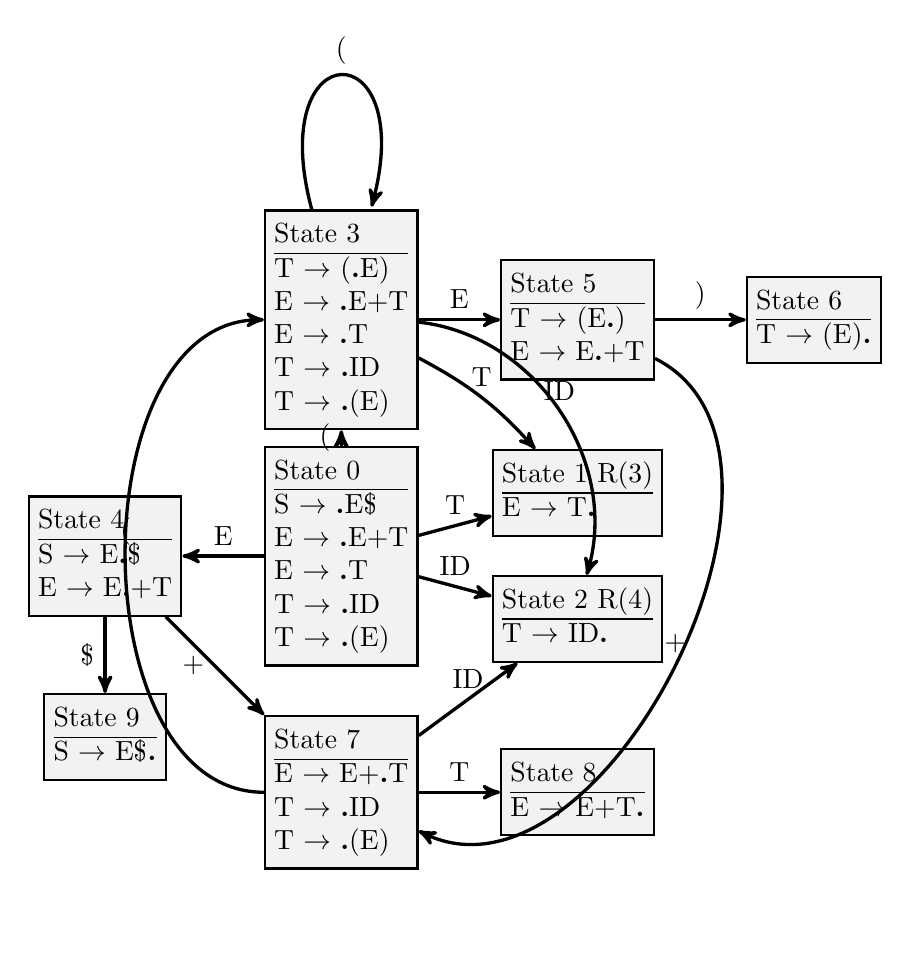
\begin{tikzpicture}
    \node[very thick, state, shape=rectangle] (0) {
    \makecell[l] {
    State 0 \\
    \hline
    S $\rightarrow$ \textbf{.}E\$ \\
    E $\rightarrow$ \textbf{.}E+T \\
    E $\rightarrow$ \textbf{.}T \\
    T $\rightarrow$ \textbf{.}ID \\
    T $\rightarrow$ \textbf{.}(E)
    }};
    \node[state, shape=rectangle, right of=0, yshift=8mm] (1) {
    \makecell[l] {
    State 1 R(3)\\
    \hline
    E $\rightarrow$ T\textbf{.}
    }};
    \node[state, shape=rectangle, below of=1, yshift=14mm] (2) {
    \makecell[l] {
    State 2 R(4)\\
    \hline
    T $\rightarrow$ ID\textbf{.}
    }};
    \node[state, shape=rectangle, above of=0] (3) {
    \makecell[l] {
    State 3 \\
    \hline
    T $\rightarrow$ (\textbf{.}E) \\
    E $\rightarrow$ \textbf{.}E+T \\
    E $\rightarrow$ \textbf{.}T \\
    T $\rightarrow$ \textbf{.}ID \\
    T $\rightarrow$ \textbf{.}(E)
    }};
    \node[very thick, state, shape=rectangle, left of=0] (4) {
    \makecell[l] {
    State 4\\
    \hline
    S $\rightarrow$ E\textbf{.}\$ \\
    E $\rightarrow$ E\textbf{.}+T
    }};
    \node[very thick, state, shape=rectangle, right of=3] (5) {
    \makecell[l] {
    State 5\\
    \hline
    T $\rightarrow$ (E\textbf{.}) \\
    E $\rightarrow$ E\textbf{.}+T
    }};
    \node[very thick, state, shape=rectangle, right of=5] (6) {
    \makecell[l] {
    State 6\\
    \hline
    T $\rightarrow$ (E)\textbf{.}
    }};
    \node[very thick, state, shape=rectangle, below of=0] (7) {
    \makecell[l] {
    State 7\\
    \hline
    E $\rightarrow$ E+\textbf{.}T \\
    T $\rightarrow$ \textbf{.}ID \\
    T $\rightarrow$ \textbf{.}(E)
    }};
    \node[very thick, state, shape=rectangle, right of=7] (8) {
    \makecell[l] {
    State 8\\
    \hline
    E $\rightarrow$ E+T\textbf{.}
    }};
    \node[very thick, state, shape=rectangle, below of=4, yshift=7mm] (9) {
    \makecell[l] {
    State 9\\
    \hline
    S $\rightarrow$ E\$\textbf{.} \\
    }};
    \draw[very thick]
          (0) edge[right, above] node{T} (1)
          (0) edge[left, above] node{ID} (2)
          (0) edge[right, left] node{(} (3)
          (0) edge[right, above] node{E} (4)
          (3) edge[bend left=10, above] node{T} (1)
          (3) edge[bend left=50, above] node{ID} (2)
          (3) edge[loop above, above] node{(} (3)
          (3) edge[right, above] node{E} (5)
          (4) edge[right, left] node{+} (7)
          (4) edge[right, left] node{\$} (9)
          (5) edge[right, above] node{)} (6)
          (5) edge[bend left=90, above] node{+} (7)
          (7) edge[right, above] node{ID} (2)
          (7) edge[bend left=90, above] node{(} (3)
          (7) edge[right, above] node{T} (8);
  \end{tikzpicture}
\end{multicols}
\subsubsection{GoTo/Action Table}
\noindent
  \begin{tabular}{|c|c|c|c|c|c|c|c|c|c|c|}
    \hline
	  & \multicolumn{8}{c|}{\textbf{Symbol}} & \\
    \hline
	  & \thead{+} & \thead{ID} & \thead{(} & \thead{)} & \thead{T} & \thead{E} & \thead{\$} & \thead{S}  & \thead{Action}\\
    \hline
	\textbf{0} &   & 2 & 3 &   & 1 & 4 &   &   & Shift \\
    \hline
	\textbf{1} &   &   &   &   &   &   &   &   & Reduce 3 \\
    \hline
	\textbf{2} &   &   &   &   &   &   &   &   & Reduce 4 \\
    \hline
	\textbf{3} &   & 2 & 3 &   & 1 & 5 &   &   & Shift \\
    \hline
	\textbf{4} & 7 &   &   &   &   &   & 9 &   & Shift \\
    \hline
	\textbf{5} & 7 &   &   & 6 &   &   &   &   & Shift \\
    \hline
	\textbf{6} &   &   &   &   &   &   &   &   & Reduce 5 \\
    \hline
	\textbf{7} &   & 2 & 3 &   & 8 &   &   &   & Shift \\
    \hline
	\textbf{8} &   &   &   &   &   &   &   &   & Reduce 2 \\
    \hline
	\textbf{9} &   &   &   &   &   &   &   &   & Accept R(1) \\
    \hline
  \end{tabular}
  \newline\newline


\end{document}
